% !TEX root = ../thesis.tex

\chapter{Applications}
\label{chap:applications}

\cleanchapterquote{It is useless to dream of revolution through content, useless to dream of a revelation through form.}{Jean Baudrillard}{(Simulacra and Simulation)}


% ------------------------------------------------------------------------------

In Chapter~\ref{chap:system}, we introduced \citeauthor{Gatys2015B}'s Neural Style algorithm for style transfer on images, showing how the knowledge acquired by pre-trained deep neural networks and the concepts behind generative models can be used to solve long-standing problems like the separation of style and content in images.

In this chapter, we will see some of the improvements that have been recently proposed to the Neural Style's style transfer method, its applicability to similar tasks of image processing, as well as other uses of generative models in perceptually challenging tasks.


% ------------------------------------------------------------------------------

\section{Style Transfer Improvements}
\label{sec:applications:improvements}

Neural Style represents the first attempt at style transfer using neural networks and it has already triggered research on improving the method further.
The Neural Style algorithm suffers two major limitations
First, performance issues derived from the fact that image generation happens as an optimization process.
And second, a perceptual quality drop when the style source is not homogeneous.
We now proceed to discuss ongoing research that tries to overcome these two flaws of the Neural Style approach

\paragraph{Performance}
As we presented in Chapter~\ref{chap:system}, the generation of stylized images is implemented in Neural Style as an optimization process, requiring forward and backward passes through the pre-trained network.
This is, unfortunately, computationally expensive and makes the style transfer algorithm unusable for real-time applications.

Both \citet{Ulyanov2016} and \citet{Johnson2016} propose, instead, training feedforward transformation networks for applying a learned style onto a given content image.
We will review \citeauthor{Johnson2016}'s solution, since it achieved better performance.
Moreover, it displayed better generalization properties, as we will see later in this chapter.

\citeauthor{Johnson2016}'s system for image transformations, based on the perceptual loss functions introduced by \citeauthor{Gatys2015B}, obtains speed-ups of three orders of magnitude in style transfer tasks when compared to Neural Style, at the same time producing compositions of comparable quality.
The system, as depicted in \autoref{sec:applications:improvements:real-time}, is composed of two sub-networks: an image transformation network and a loss network.
On the one hand, the image transformation network is a deep residual convolutional neural network \cite{He2015}, allowing more efficient learning than traditional convolutional networks.
On the other hand, the loss network is a pre-trained VGG-16 network, similar to the VGG-19 network used by Neural Style.

\begin{figure}[t]
  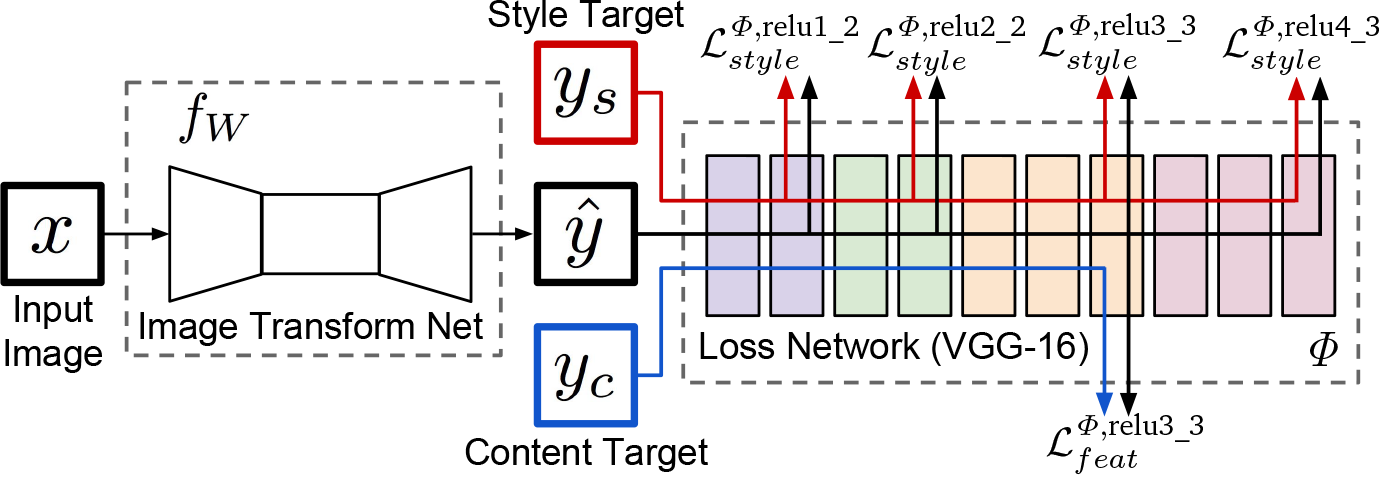
\includegraphics[width=\textwidth]{gfx/app-real-time}
  \caption{
    Overview of \citeauthor{Johnson2016}'s system for image transformation \cite{Johnson2016}.
    The system is composed of an image transformation network $f_W$ and a loss network $\mathit{\Phi}$.
    The image transformation network receives an input image $x$ to produce a transformed image $\hat{y}$.
    The loss network receives the transformed image, a style target $y_s$, and a content target $y_c$.
    It then calculates the feature loss $\mathcal{L}_{feat}$ and the style loss $\mathcal{L}_{style}$ at different stages.
  }
  \label{sec:applications:improvements:real-time}
\end{figure}

The network training is performed by repeating the following process several times.
A content image $x$ is given to the image transformation network, which produces a transformed image $\hat{y}$.
This transformed image is fed to the loss network with the style source $y_s$ we want the network to learn and the original content image as $y_c$.
The loss network calculates the the feature loss $\mathcal{L}_{feat}$ as well as the style loss $\mathcal{L}_{style}$ and both are used in the loss function for adjusting the weights of the transformation network.
Following this procedure, the image transformation network effectively learns how to transfer a particular style onto the given content images in a simple feedforward pass.

\paragraph{Perceptual Quality}
As highlighted both by \citet{Nikulin2016} and \citet{Yin2016}, Neural Style seamlessly transfers the style only if it is highly repetitive and homogeneous over the whole style image.
Because the style representation is taken over the whole image, the style reconstruction fails to capture local style details like particular face features or different textures in background and foreground.
In consequence, perceptual quality drops as these details get averaged out when transferred onto the content image.

\citeauthor{Nikulin2016}'s analysis of Neural Style concludes by proposing an untested style-content global covariation loss function that would potentially result in content-aware style transfer, but they also anticipate its computational infeasibility.

Independently, \citeauthor{Yin2016} proposes a semi-automatic procedure to ensure content-aware style transfer, as we show in \autoref{sec:applications:improvements:content-aware}.
We can observe a real painting of a hummingbird on wood board as the style source and a photograph of a hummingbird on a white background.
Making the photograph display the local style properties of the painting on the same local spots would be desired.
However, Neural Style produces a washed-out composition of low perceptual quality where the style of the background creeps into the foreground.
The content-aware approach preserves the perceptual details of the photograph while applying the style from the painting.

\begin{figure}[t]
  \captionsetup[subfigure]{labelformat=empty}
  \begin{subfigure}[b]{0.244\textwidth}
    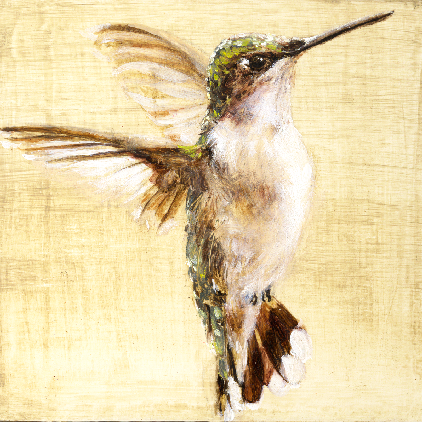
\includegraphics[width=\textwidth]{gfx/app-content-aware-1}
  \end{subfigure}
  \begin{subfigure}[b]{0.244\textwidth}
    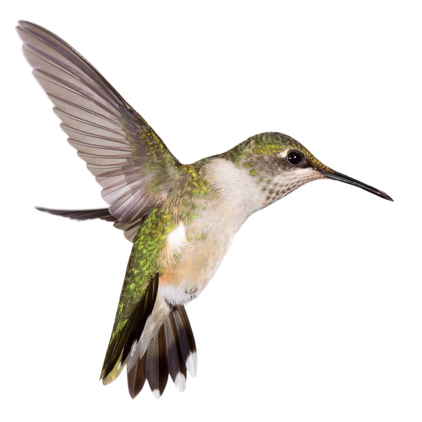
\includegraphics[width=\textwidth]{gfx/app-content-aware-2}
  \end{subfigure}
  \hfill
  \begin{subfigure}[b]{0.244\textwidth}
    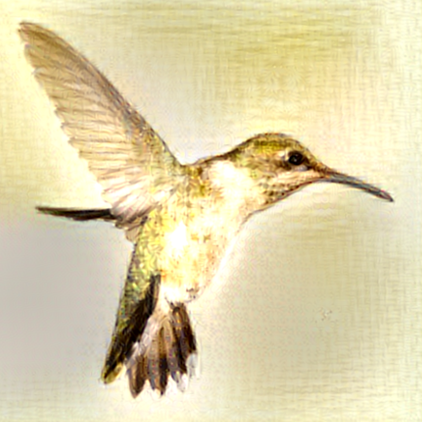
\includegraphics[width=\textwidth]{gfx/app-content-aware-3}
  \end{subfigure}
  \begin{subfigure}[b]{0.244\textwidth}
    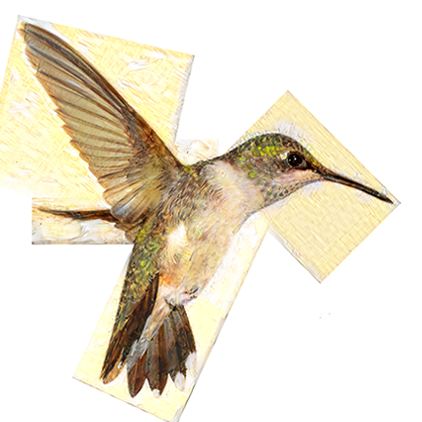
\includegraphics[width=\textwidth]{gfx/app-content-aware-4}
  \end{subfigure}
  \par\smallskip
  \begin{subfigure}[b]{0.244\textwidth}
    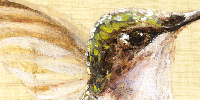
\includegraphics[width=\textwidth]{gfx/app-content-aware-5}
    \caption{Style}
  \end{subfigure}
  \begin{subfigure}[b]{0.244\textwidth}
    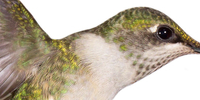
\includegraphics[width=\textwidth]{gfx/app-content-aware-6}
    \caption{Content}
  \end{subfigure}
  \hfill
  \begin{subfigure}[b]{0.244\textwidth}
    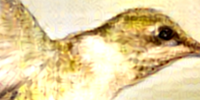
\includegraphics[width=\textwidth]{gfx/app-content-aware-7}
    \caption{Neural Style}
  \end{subfigure}
  \begin{subfigure}[b]{0.244\textwidth}
    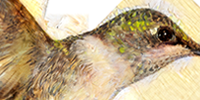
\includegraphics[width=\textwidth]{gfx/app-content-aware-8}
    \caption{Context-Aware}
  \end{subfigure}
  \caption{
    Comparison of Neural Style and content-aware style transfer \cite{Yin2016}.
  }
  \label{sec:applications:improvements:content-aware}
\end{figure}

\citeauthor{Yin2016}'s content-aware procedure consists in the following steps.
First, manually segmenting overlapping parts of the foreground content image, being them the head, tail, and wings in this example.
Then, content segments are matched with the local style segments and subsequently processed with the content-aware style transfer algorithm.
The main difference of the algorithm compared to Neural Style is that, instead of a white noise image, the content segment is the initial image used to start generating the stylized version.
In this way, the algorithm preserves more pixels of the original content image.
Finally, the resulting stylized segments are simply merged together in the overlapping region.


% ------------------------------------------------------------------------------

\section{Style Transfer Uses}
\label{sec:applications:uses}

In this section, we describe two image processing methods inspired by the methods in the Neural Style algorithm.
One of them simply applies style transfer to videos, while the other uses the perceptual loss proposed by \citeauthor{Gatys2015B} for super-resolution.

\paragraph{Neural Style Video}
The first obvious extension of Neural Style is applying it on the different frames of a video to obtain an stylized version of the original video.
But one of the problems with the naive approach of transferring the style to each frame of the video independently is that it results in notable flickering.
This occurs due to Neural Style being initialized with a randomly generated white noise image and, therefore, two consecutive frames easily end up converging to very different local minima in the optimization process.

\citet{Ruder2016} proposes a system that prevents flickering, among other artifacts, by introducing a temporal constraint that penalizes deviations between consecutive frames and produces smooth transitions.
\autoref{sec:applications:uses:video} compares the results obtained by processing each video frame independently and by using \citeauthor{Ruder2016}'s constrained-based algorithm, which are best observed in the video available at \url{https://youtu.be/vQk_Sfl7kSc}.

Watching this video, it can be appreciated how colors are randomly assigned for each frame when processed independently, whereas both the foreground and the background maintain coherent colors throughout the video using \citeauthor{Ruder2016}'s constrained optimization.

\begin{figure}[t]
  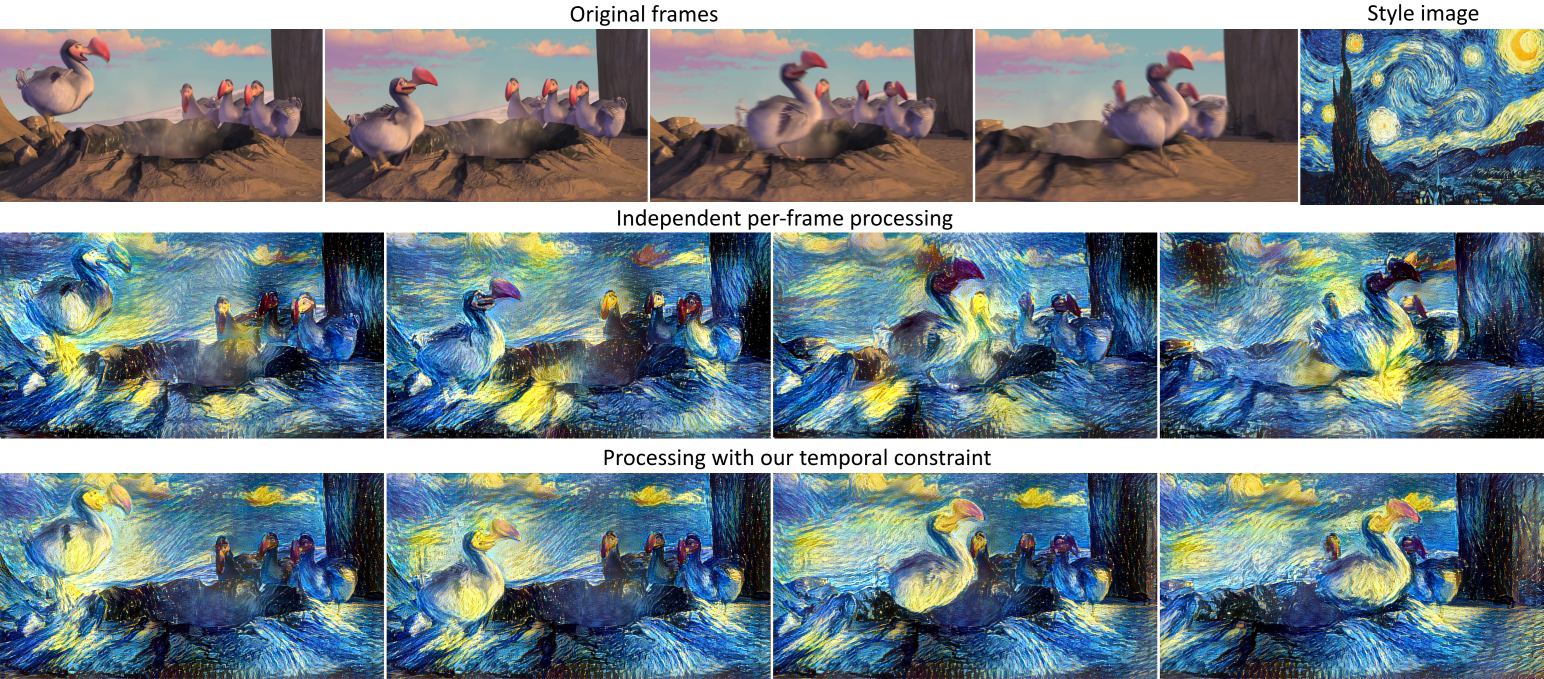
\includegraphics[width=\textwidth]{gfx/app-neural-video}
  \caption{
    Scene from Ice Age (2002) processed using the style of Van Gogh's The Starry Night \cite{Ruder2016}.
    Comparison of independent per-frame style transfer to the time constraint approach.
    Comparing independent per-frame processing to the time constraint approach.
    Flickering can be appreciated in the former as the colors of the dodo change from frame to frame.
  }
  \label{sec:applications:uses:video}
\end{figure}

\citeauthor{Ruder2016}'s system solves flickering by initializing the style transfer algorithm for a given frame with the previous stylized frame.
This alone achieves that, during the loss optimization process, unchanged areas are found to be already optimized and do not need to change, while the rest of the frame is rebuilt.
The method can be made robust against scenes with motion by calculating the optical flow of the frame and warping the pixels of the stylized frame in that direction before feeding it to the style transfer algorithm as its initial image.
In addition, they include an explicit per-pixel temporal consistency loss to encourage stronger consistency between consecutive frames during the optimization process.

\paragraph{Super-resolution}
As we mentioned before, \citeauthor{Johnson2016}'s architecture for learning style transfer enables it for other image processing problems.
Super-resolution is one of them.
The goal of super-resolution is, given a low resolution image, to produce a larger resolution version.
Recent methods typically train convolutional neural networks using a per-pixel loss function between the output and ground-truth images \cite{Dong2016}.
Instead, \citeauthor{Johnson2016}'s image transformation network can learn how to apply super-resolution using high-level features by using the perceptual content loss used in Neural Style, producing more compelling details than the state-of-the-art methods.

Like in style transfer tasks, there is no single correct output, as there are many high-resolution images that could have generated the same low-resolution input, and, therefore, semantic reasoning helps producing features that are more visually meaningful to humans.
By using the VGG-16 network pre-trained for object recognition as the loss network, the image transformation network is capable of inferring fine details from the visually ambiguous low-resolution inputs.

\autoref{sec:applications:uses:super-res} compares super-resolution results obtained using per-pixel loss and feature loss functions.
We can observe how bicubic interpolation, a simple mathematical operation, produces very blurry results.
Comparatively, state-of-the-art deep neural network minimizing per-pixel loss $\mathcal{L}_{pixel}$, although objectively superior to the other approaches, do not yield more compelling result.
\citeauthor{Johnson2016}'s approach recreates fine details, as we can clearly see the horses' legs and their hooves.

\begin{figure}[t]
  \begin{subfigure}[b]{0.244\textwidth}
    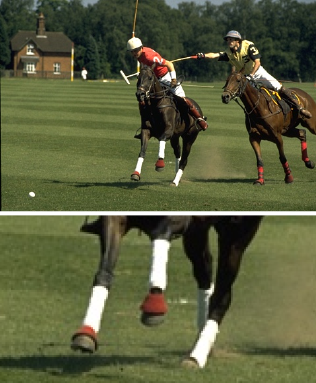
\includegraphics[width=\textwidth]{gfx/app-super-res-1}
    \caption{Ground Truth}
  \end{subfigure}
  \begin{subfigure}[b]{0.244\textwidth}
    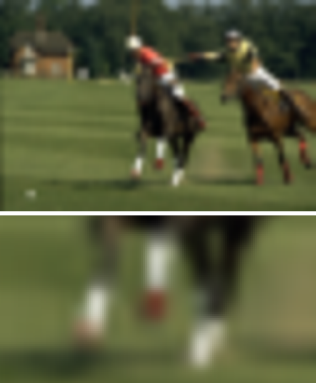
\includegraphics[width=\textwidth]{gfx/app-super-res-2}
    \caption{Bicubic}
  \end{subfigure}
  \hfill
  \begin{subfigure}[b]{0.244\textwidth}
    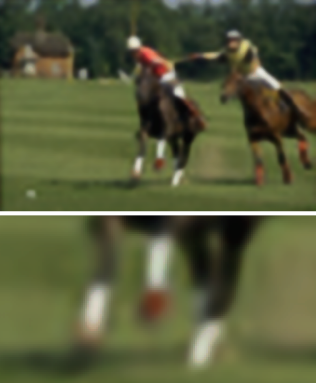
\includegraphics[width=\textwidth]{gfx/app-super-res-3}
    \caption{$\mathcal{L}_{pixel}$}
  \end{subfigure}
  \begin{subfigure}[b]{0.244\textwidth}
    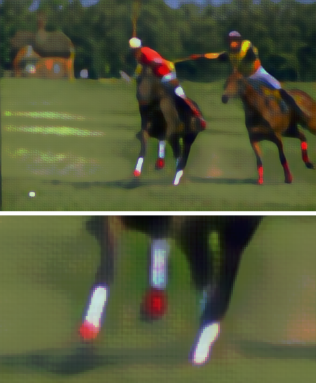
\includegraphics[width=\textwidth]{gfx/app-super-res-4}
    \caption{$\mathcal{L}_{feat}$}
  \end{subfigure}
  \caption{
    Comparison of super-resolution techniques \cite{Johnson2016}.
    Given a low-resolution version of an original image (a), both bicubic method (b) and per-pixel loss function in deep neural networks (c) produce blurry results.
    Using feature loss to train a network for supersampling (d), finer details are inferred.
  }
  \label{sec:applications:uses:super-res}
\end{figure}

If we look again at \autoref{sec:applications:improvements:real-time}, the training process of the image transformation network for a particular super-resolution factor (e.g. $\times{2}$, $\times{4}$, $\times{8}$) works in the following way.
An image $x$, down-sampled accordingly to the factor to be learnt, is given to the image transformation network and produces a transformed image $\hat{y}$.
The loss network receives the image at the original resolution $y_c$ to calculate the feature loss.
No style loss needs to be calculated in this case, so the loss network calculates the the feature loss $\mathcal{L}_{feat}$ alone.
The image transformation network, by minimizing the feature loss, effectively learns how to apply super-resolution at the desired factor to the given images while maintaining their high-level features.


% ------------------------------------------------------------------------------

\section{Beyond Neural Style}
\label{sec:applications:beyond}

Finally, we present two more novel techniques that use deep neural networks to solve perceptive problems: the colorization of grayscale images and the visual segmentation of concepts in images.

\paragraph{Colorization}
The colorization of grayscale images is also a unconstrained problem, like super-resolution.
Given a grayscale image, there are many differently-colored versions that could have produced it.
Colorization methods try to generate a set of colors that result believable to a human observer and, therefore, classical approaches typically require significant user interaction.

More recently, fully-automatic colorization algorithms have been proposed using deep neural networks.
They model the problem as a regression problem against per-pixel ground truth colors \cite{Cheng2015}.
Their results, however, present desaturated colors.
\citet{Zhang2016} propose a system that approaches the colorization task as a semantic classification problem, relying on perceptual reasoning, and produces vibrant and realistic colorizations, capable of fooling human observers in a color Turing test better than any other method to date.

\autoref{sec:applications:beyond:color} shows a comparison between the regression approach and \citeauthor{Zhang2016}'s classification approach for grayscale colorization.
More examples are available at \url{http://richzhang.github.io/colorization/}.
As it can be noted, the colors produced by the classification approach do not necessarily match the ground truth, but are more vibrant and believable than those generated through regression.

\begin{figure}[t]
  \captionsetup[subfigure]{labelformat=empty}
  \begin{subfigure}[b]{0.244\textwidth}
    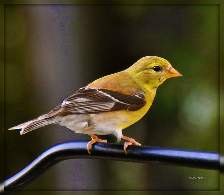
\includegraphics[width=\textwidth]{gfx/app-color-1}
    \caption{Ground Truth}
  \end{subfigure}
  \begin{subfigure}[b]{0.244\textwidth}
    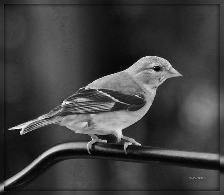
\includegraphics[width=\textwidth]{gfx/app-color-2}
    \caption{Input}
  \end{subfigure}
  \hfill
  \begin{subfigure}[b]{0.244\textwidth}
    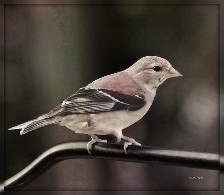
\includegraphics[width=\textwidth]{gfx/app-color-3}
    \caption{Regression}
  \end{subfigure}
  \begin{subfigure}[b]{0.244\textwidth}
    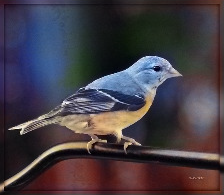
\includegraphics[width=\textwidth]{gfx/app-color-4}
    \caption{Classification}
  \end{subfigure}
  \caption{
    Automatic grayscale image colorization \cite{Zhang2016}.
    Comparison between regression-based and classification-based colorization, the latter producing more vibrant colors.
  }
  \label{sec:applications:beyond:color}
\end{figure}

The system consists of a feedforward pass in a convolutional neural network.
For each pixel of a given grayscale image, a color is inferred based on it semantic classification.
The network, trained over the million color images in ImageNet, is capable of per-pixel classification as it has learned the dependencies between the semantics and the textures of grayscale images and their color versions.

Training the network alone did not ensure the generated colors would come out vividly in the generated image.
Caused by non-saturated pixels being orders or magnitude more abundant than saturated ones in ImageNet, the network is more likely to propose the former.
This asymmetry is expected, as image backgrounds tend to be in the spectrum of non-saturated colors and, therefore, color probabilities are normalized to incentivize foreground, more saturated colors.

Finally, \citeauthor{Zhang2016}'s network can produce more vibrant colors than prior approaches because they quantize the color space in buckets.
The Euclidean distance is generally used to measure the loss between a generated image and its ground truth.
This, however, favors gray tonalities.
For instance, if an object can be red or green (e.g. an apple), the ``correct'' color using the Euclidean distance should fall in between, but would never be the pure red nor the pure green.
Instead, by using color buckets, when the predicted color falls in the bucket of the red color space, the Euclidean distance is simply measured with respect to the correct tonality of red, not being affected at all by the possibility of green also being a correct color.

\paragraph{Semantic Segmentation}
Image semantic segmentation is the task of partitioning an image into coherent sections.
Traditionally, this was done without actually understanding the semantics of the image, rather by using handcrafted features like color or brightness variations.

\begin{figure}[t]
  \captionsetup[subfigure]{labelformat=empty}
  \begin{subfigure}[b]{0.244\textwidth}
    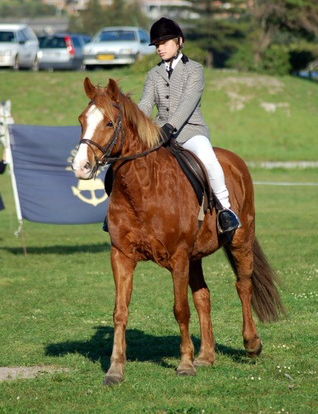
\includegraphics[width=\textwidth]{gfx/app-segmentation-1}
    \caption{Image}
  \end{subfigure}
  \begin{subfigure}[b]{0.244\textwidth}
    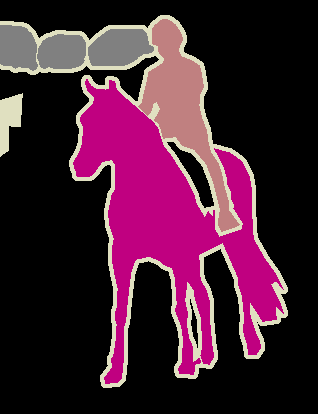
\includegraphics[width=\textwidth]{gfx/app-segmentation-2}
    \caption{Ground Truth}
  \end{subfigure}
  \hfill
  \begin{subfigure}[b]{0.244\textwidth}
    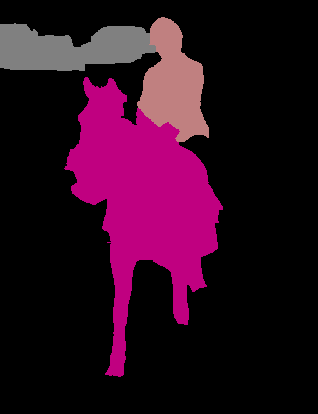
\includegraphics[width=\textwidth]{gfx/app-segmentation-3}
    \caption{SDS \cite{Hariharan2014}}
  \end{subfigure}
  \begin{subfigure}[b]{0.244\textwidth}
    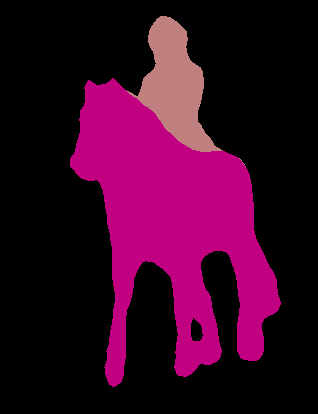
\includegraphics[width=\textwidth]{gfx/app-segmentation-4}
    \caption{FCN \cite{Long2015}}
  \end{subfigure}
  \caption{
    Semantic segmentation \cite{Long2015}.
    Comparison between ground truth, Simultaneous Detection Segmentation (SDS), and Fully Convolutional Network (FCN) results.
  }
  \label{fig:sec:applications:beyond:segmentation}
\end{figure}

Convolutional neural networks have been used for per-pixel classification \cite{Farabet2013,Hariharan2014}, but did not generalize well, as they required pre- and post- processing.
\citet{Long2015} proposes a fully convolutional network for semantic segmentation that adapts contemporary classification networks to transfer their learned representations, does not require pre- nor post-processing, is more efficient, and exceeds state-of-the-art performance.

\autoref{fig:sec:applications:beyond:segmentation} shows \citeauthor{Long2015}'s Fully Convolutional Network (FCN) results compared with the previous state of the art Simultaneous Detection Segmentation (SDS) \cite{Hariharan2014}.
We can see how the whole shape of the horse with its rider was recovered, and how even finer structures like the legs are intact.

\citeauthor{Long2015}'s system can be implemented by converting any convolutional network, already pre-trained for object recognition, into a fully-convolutional network, and fine-tuning it for semantic segmentation.

By converting the original convolutional network, with fully-connected layers, into a fully-convolutional, without fully-connected layers, the network looses its ability to classify.
Conversely, the network is then capable of producing transformed images in the last layer.
The fine-tuning step consists of re-training the later layers of the network, which are more relevant to the task at hand, without discarding the learned weights in the earlier layers, which already know how to extract general purpose visual features.
Semantic segmentation can be attained by training with the PASCAL VOC 2011 dataset, containing ground truth for segmentation tasks.

Finally, putting everything together, by applying fine-tuning with the PASCAL VOC dataset and a per-pixel loss function, the pre-trained, now fully-convolutional network is effectively trained so that the last layer produces the per-pixel class predictions observable in \autoref{fig:sec:applications:beyond:segmentation}.
